\documentclass[12pt]{report}
\usepackage[utf8]{inputenc}
\usepackage{amsmath}
\usepackage{amsfonts}
\usepackage{venndiagram}
\usepackage{hyperref}
\usepackage{multirow}
\usepackage{graphicx}
\usepackage{geometry}
\usepackage{subcaption}
\usepackage{hyperref}
\usepackage{float}
\usepackage{amsmath}%
\usepackage{MnSymbol}%
\usepackage{wasysym}%
\geometry{margin=1.1in}
\begin{document}
\begin{titlepage}
   \begin{center}
       \vspace*{5cm}

       \textbf{\huge{No Waste}}

       \vspace{0.5cm}
        \href{https://github.com/UniRoby/Recipe_Suggester_RSAI}{GitHub}
            
       \vspace{1.5cm}

       \textbf{Roberto Piscopo, 0512109906  \\ Alessandro Satta, 0512110929}

       \vfill

       
\includegraphics[width=0.4\textwidth]{img/logo.png}
            
       Dipartimento di Informatica\\
       Università degli studi di Salerno\\
       13/02/2023         
   \end{center}
\end{titlepage}

\tableofcontents

\chapter{Introduzione}
\section{Contesto}    
Il progetto nasce dal problema che molte persone hanno, ovvero avere in dispensa/frigo degli ingredienti dimenticati oppure accumulati e non sapere cosa cucinare. Oppure banalmente ottenere nuove idee per delle ricette in base ad altre che ci piacciono.

\section{Idea}
Il nostro progetto ha lo scopo di creare un agente intelligente capace di consigliare una o più ricette in base a quello che l’utente ha a disposizione, o che gli piace.

\chapter{PEAS}
\section{Specifiche}
La prima cosa da fare quando si progetta un agente intelligente è la definizione delle Specifiche Peas.
\begin{itemize}
\item[] $\blacksquare$  \textbf{Performance:} Migliore ricetta in base agli ingredienti forniti

\item[] $\blacksquare$  \textbf{Enviroment:} L’ambiente nel quale il nostro agente opera è composto da tutte le ricette del dataset con i relativi: titolo, ingredienti, ratings, tempo di preparazione, istruzioni, tipologia.

L’ambiente risulta:

\begin{itemize}
\item \textbf{Completamente osservabile:} si ha accesso a tutte le informazioni di ogni ricetta
\item \textbf{Deterministico:} L'ambiente deterministico significa che l'agente sa esattamente cosa aspettarsi in base alle informazioni fornite e agli input dell'utente. In altre parole, l'agente sa che dati gli stessi input, otterrà sempre lo stesso output, l'agente sa che se gli vengono forniti gli stessi ingredienti, troverà sempre la stessa ricetta migliore nell'ambiente statico
\item \textbf{Episodico:} l'agente si trova in un singolo episodio in cui riceve gli ingredienti in input e restituisce la migliore ricetta come output, senza alcuna interazione ulteriore con il mondo esterno.
\item \textbf{Statico:} L’insieme delle ricette e le relative informazioni non cambiano nel corso del tempo
\item \textbf{Discreto:} L’agente ha a disposizione un numero limitato di azioni
\item \textbf{Singolo Agente:} è presente solo un agente che opera nell’ambiente
 \end{itemize}


$\blacksquare$\textbf{Attuatori:} L'algoritmo utilizzato per generare le possibili soluzioni e selezionare la migliore. 

$\blacksquare$\textbf{Sensori:} Gli input dell'utente, ovvero la lista degli ingredienti.
 \end{itemize}


\chapter{Dataset}
\section{Creazione Dataset}
Non esistendo dei dataset di ricette in italiano, abbiamo dovuto crearlo noi. Per farlo abbiamo utilizzato la tecnica del Web Scraping, ovvero una tecnica tramite la quale estrarre dati da un sito web, nel nostro caso da \href{https://www.giallozafferano.it/}{GialloZafferano}. 
Abbiamo utilizzato una libreria di python chiamata recipe-scrapers insieme alla libreria BeautifulSoup  
BeautifulSoup è stato utilizzata per prendere tutti i link delle ricette delle 426 pagine di GialloZafferano.
    \begin{figure}[H]
        \centering
        {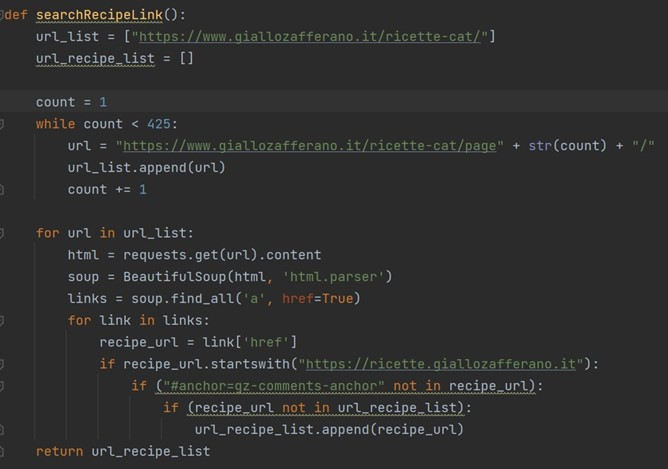
\includegraphics[width=0.9\textwidth]{img/img1.jpg}}
    \end{figure}
Dopodichè  per ogni pagina di una ricetta sono state usate le funzioni di recipe scrapers per ottenere le feature da inserire nel dataset quali: titolo ricetta, tempo preparazione, valutazione, categoria/tipologia, istruzioni.
    \begin{figure}[H]
        \centering
        {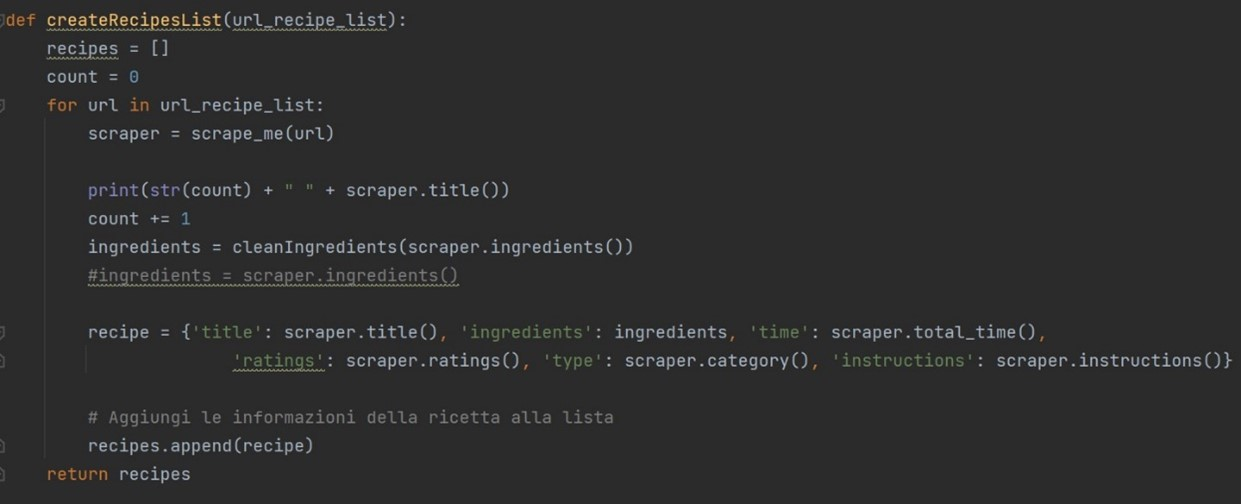
\includegraphics[width=0.9\textwidth]{img/img2.jpg}}
    \end{figure}
Poi tutte le ricette sono state salvate in un file csv
    \begin{figure}[H]
        \centering
        {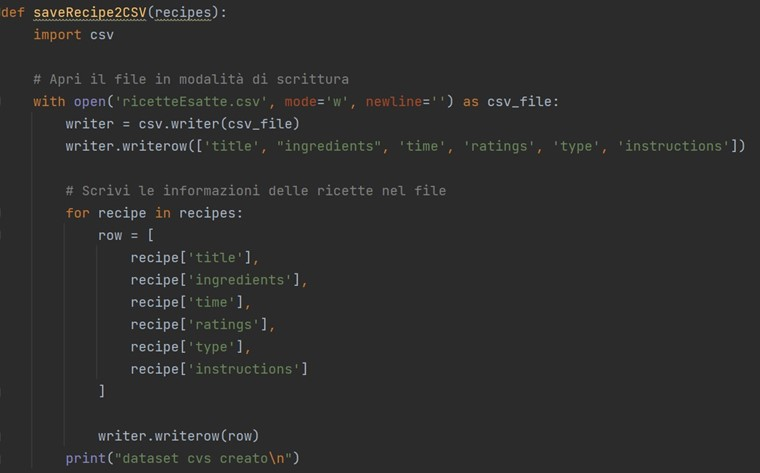
\includegraphics[width=0.9\textwidth]{img/img3.jpg}}
    \end{figure}



\section{Data Understanding, Data Preparation \& Data Cleaning}
Abbiamo creato un programma per l’esplorazione del dataset in modo tale da effettuare il conteggio delle ricette, del tempo medio per la preparazione , del numero di ricette per tipologia, del numero di ingredienti totali, del numero di ingredienti più usati, di quelli meno usati, del conteggio per ogni singolo ingrediente. 

Un primo problema si è presentato con la lista degli ingredienti. Se prediamo ad esempio la ricetta “Tiramisù” i suoi ingredienti sono: 

\textbf{Mascarpone} 750 g

\textbf{Uova}(freschissime, circa 5 medie) 260 g

\textbf{Savoiardi} 250 g

\textbf{Zucchero} 120 g

\textbf{Caffè}(della moka, zuccherato a piacere) 300 g

A noi interessano solo i nomi degli ingredienti, in quanto saranno utilizzati per trovare ricette simili dati degli ingredienti in input. Quindi andavano cancellate tutte le grammature e altre informazioni non necessarie come “freschissime, circa 5 medie”.

Per fare questo è stato creato un programma in python che andava a rimuovere le grammature, i numeri, informazioni nelle parentesi ed informazioni di contorno in generale. Inoltre bisognava anche andare a sostituire alcuni ingredienti composti usando solo l’ingrediente principale ad esempio: Estratto di vaniglia, doveva diventarevaniglia. 

Poi sono stati rimossi tutti i caratteri non necessari come: [,](,) /, ecc

Sono stati rimossi tutti quei dettagli come “piccola”. E se ci sta piccolo o piccoli ? Abbiamo rimosso tutte le varianti manualmente, (solo dopo siamo venuti a conoscenza di funzioni automatiche di lemmatizzazione e stemming).

Tutti gli ingredienti sono stati portati in lower Case.

Fatto ciò la lista di ingredienti pulita è stata salvata come stringa ed inserita al posto della lista di ingredienti precedente alla pulizia. Alla fine del processo veniva creato un novo dataset.

La fase di pulizia del dataset però non finiva qui.

Grazie al conteggio per ogni singolo ingrediente dell'espolorazione dataset aggiornato, ci ha permesso di pulire ulteriormente il dataset da ricette superflue. Difatti abbiamo eliminato circa un centinaio di ricette che avevano ingredienti unici, troppo specifici che non ci avrebbero aiutato nell’identificazione di ricette simili, in quanto uniche nel loro genere. (Per il codice vedere removeRow.py in RecipeScraper)

\begin{figure}[H]
        \centering
        {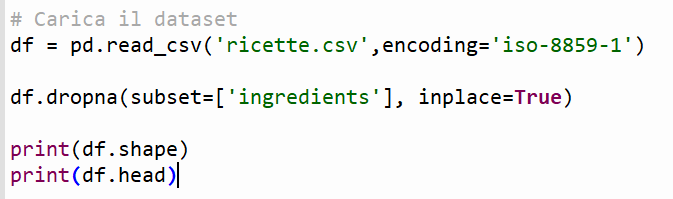
\includegraphics[width=0.9\textwidth]{img/img4.jpg}}
\end{figure}
[6037 rows x 6 columns]

 Il nostro dataset ha poco più di 6000 ricette ed è un file CSV.

\begin{figure}[H]
        \centering
        {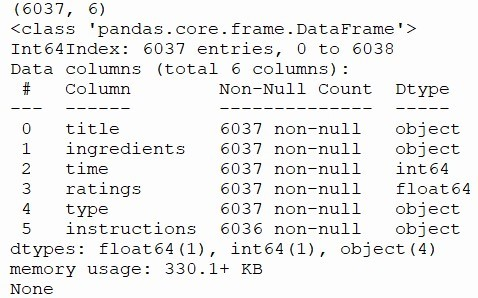
\includegraphics[width=0.8\textwidth]{img/img5.jpg}}
\end{figure}


Esempio prime righe…

\begin{center}
\resizebox{\columnwidth}{!}{\begin{tabular}{|p{0.1\linewidth}|p{0.22\linewidth}|c|c|c|p{0.25\linewidth}|} 
 \hline
 Titolo & Ingredienti & tempo & Valutazione & Tipologia & Istruzioni \\ [0.5ex] 
 \hline
Tiramisù  & mascarpone,uova,\par savoiardi,zucchero,\par caffè,cacao & 46 & 4.2 & Dolci & Per preparare il \par tiramisù preparate il caffé... \\
 \hline
Spaghetti alla\par carbonara & spaghetti,guanciale,\par uova,pecorino,pepe & 25 & 4.2 & Primi piatti  & Per preparare gli spaghetti alla\par carbonara...  \\
\hline
\multicolumn{6}{|c|}{ecc...} \\
 \hline
\end{tabular}}
\end{center}

Conteggio ingredienti è stato fatto sia con la libreria nltk sia con la libreria csv leggendo le righe: 

\begin{figure}[H]
  \centering
  \begin{subfigure}[b]{0.45\linewidth}
    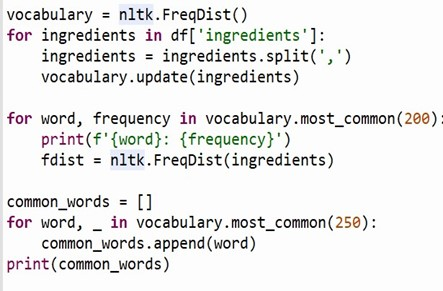
\includegraphics[width=\linewidth]{img/img6.jpg}
  \end{subfigure}
  \begin{subfigure}[b]{0.45\linewidth}
    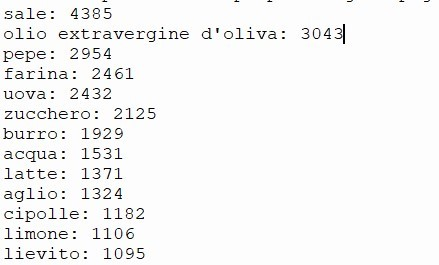
\includegraphics[width=\linewidth]{img/img7.jpg}
  \end{subfigure}
\end{figure}

Conteggio ricette per Tipologia :

\begin{figure}[H]
  \centering
  \begin{subfigure}[b]{0.9\linewidth}
    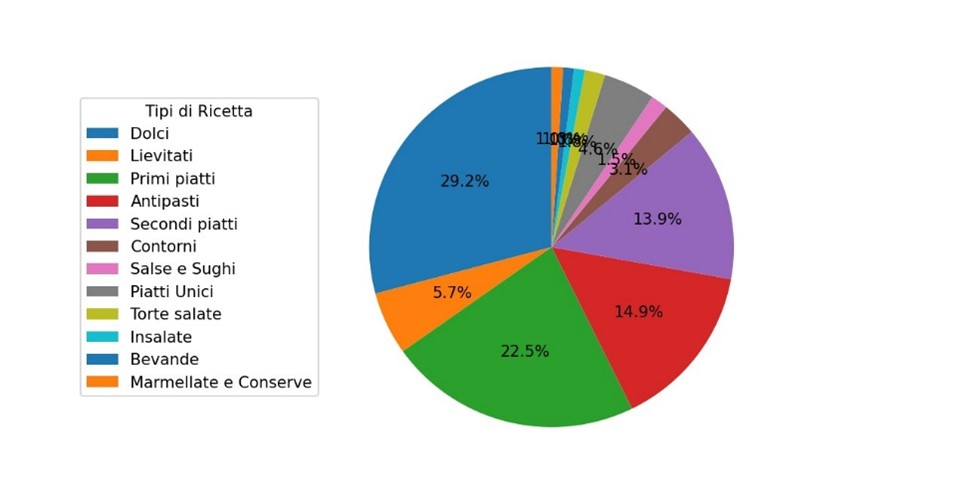
\includegraphics[width=\linewidth]{img/img8.jpg}
  \end{subfigure}
  \begin{subfigure}[b]{0.5\linewidth}
    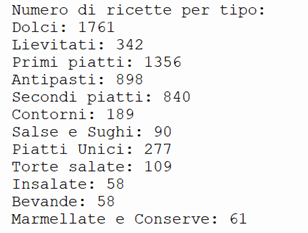
\includegraphics[width=\linewidth]{img/img9.jpg}
  \end{subfigure}
\end{figure}
\section{Feature Scaling}
Non c’erano dati particolarmente discordanti e quindi non c’è stato bisogno di scalare e normalizzare. 
\section{Feature Selection}
Come già detto , il dataset delle ricette è stato creato e quindi di seguito vengono spiegati i motivi di ogni caratteristica:
\begin{itemize}
	\item Titolo: è utile per mostrare all’utente la ricetta consigliata .
	\item Ingredienti: è la feature dominante in quanto ci permette di capire se due ricette sono simili.
	\item Rating: utile per capire se una determinata ricetta piace agli utenti o meno (non verrà usata nella soluzione finale).
	\item Prep\_time:è utile per capire il tempo di preparazione della ricetta.
	\item Categoria: è utile per capire la tipologia della ricetta.
 \end{itemize}

\chapter{Prima Soluzione : Algoritmi genetici}
Abbiamo provato a realizzare un agente intelligente attraverso gli Algoritmi Genetici. (per il codice vedere cartella GA) (Dataset Vecchio utilizzato : id, title, ingredients, likes, prep\_time, Solo 300 ricette)

Un GA è una proceduta ad alto livello (meta-euristica) ispirata alla genetica per definire un algoritmo di ricerca. Evolve una popolazione di individui (soluzioni candidate) producendo di volta in volta soluzioni sempre migliori rispetto ad una funzione obiettivo, fino a raggiungere l’ottimo o un’altra condizione di terminazione. La creazione di nuove generazioni di individui avviene applicando degli operatori genetici, precisamente selezione, crossover e mutazione.

\textbf{Nel nostro caso le caratteristiche del GA erano le seguenti:}
Codifica individuo (ricetta) era formata da un array di 8 interi che potevano assumere il valore solo di 0 o 1. L’intero individuo andava ad individuare l’indice di una riga del dataset e quindi di una ricetta.

\textbf{Size popolazione}: 5

\textbf{Selezione}: abbiamo usato la tecnica dei Steady-State GA, invece di generare nuove generazioni si va a migliorare costantemente quella attuale. Si selezionano i due migliori individui come genitori

\textbf{Crossover}: il crossover (Single/Two-Point) avviene tra i due genitori selezionati al punto precedente. Il nuovo individuo andrà a sostituire il peggiore della popolazione. Nel caso in cui si va a creare un individuo già esistente nella popolazione allora si applica la mutazione (bit flip)

\textbf{Stopping condition}: terminiamo l’evoluzione quando si superano le 500 iterazioni o quando si è raggiunta una certa fitness.

\textbf{La funzione di fitness} è data dal numero di ingredienti in comune con quelli inseriti moltiplicati per i likes  il tutto diviso per il tempo di preparazione.

Dopo varie prove e modifiche agli operatori genetici ci siamo resi conto che l’algoritmo era un po' troppo casuale. Molte volte trovava le due migliori ricette in una 50ina di generazioni altre volte arrivava fino a 500 iterazioni trovando due ricette con fitness molto basse.

\begin{figure}[H]
        \centering
        {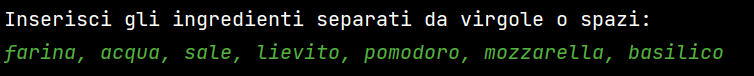
\includegraphics[width=0.9\textwidth]{img/img35.jpg}}
\end{figure}

\begin{figure}[H]
        \centering
        {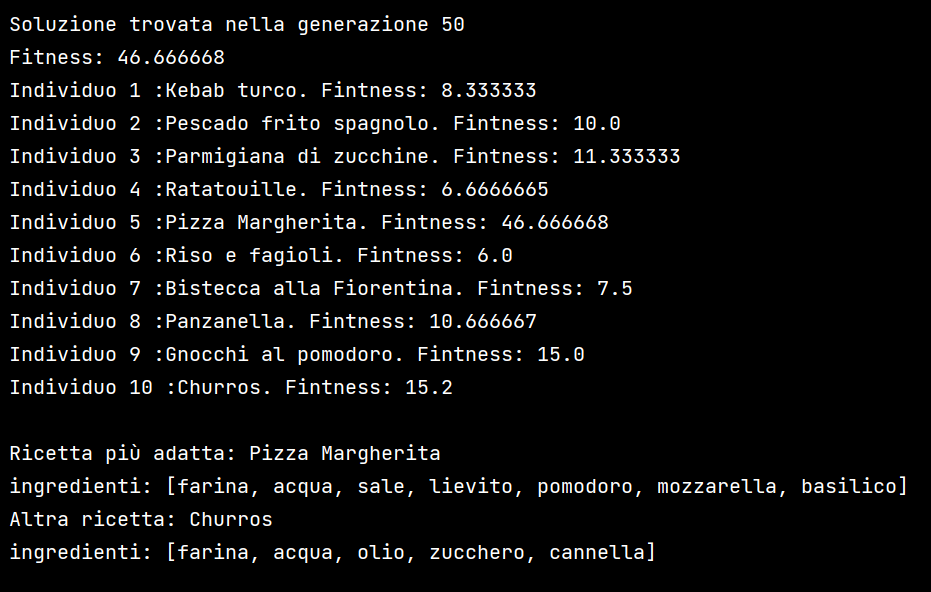
\includegraphics[width=0.9\textwidth]{img/img34.jpg}}
\end{figure}

Così abbiamo pensato che la codifica non era adatta o probabilmente non era adatto al nostro problema un algoritmo Genetico.

\chapter{Seconda Soluzione : Algoritmo A*}

Quindi abbiamo optato per un algoritmo di ricerca informata. Il più utilizzato tra gli algoritmi di ricerca informata è l’A*. (Dataset Vecchio utilizzato : id, title, ingredients, likes, prep\_time, Solo 300 ricette)

Per il codice vedere la cartella AStar

\textbf{L'algoritmo A*} è un algoritmo di ricerca che utilizza una funzione di valutazione per determinare la distanza tra un nodo corrente e un nodo obiettivo. In questo caso, la funzione di valutazione è "evaluate\_recipe" che valuta una singola ricetta sulla base di quanti ingredienti corrispondono a quelli forniti in input e sulla base del numero di likes della ricetta.

La funzione \textbf{"evaluate\_recipe"} valuta una singola ricetta in base agli ingredienti forniti in input. La funzione utilizza un ciclo for per verificare se ciascun ingrediente della ricetta è presente negli ingredienti forniti in input. Se un ingrediente è presente, la valutazione della ricetta viene incrementata di 1. Inoltre, la valutazione della ricetta viene incrementata anche dal numero di "likes" della ricetta diviso 100,per normalizzare i "likes"
\begin{figure}[H]
        \centering
        {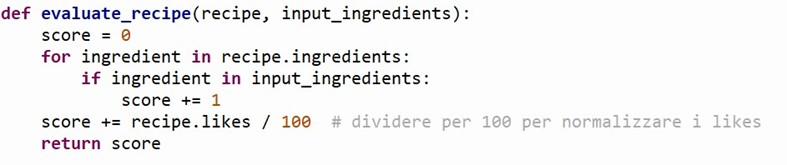
\includegraphics[width=0.9\textwidth]{img/img10.jpg}}
\end{figure}

La funzione \textbf{"find\_best\_recipe"} utilizza l'algoritmo A* per trovare la migliore ricetta possibile. Inizia creando due liste: "open\_list" e "closed\_list". "open\_list" contiene tutte le ricette del dataset all'inizio, mentre "closed\_list" è vuota.

All'interno del ciclo while, l'algoritmo seleziona la ricetta con la valutazione più alta dalla lista "open\_list" e la sposta nella lista "closed\_list". Successivamente, verifica se tutti gli ingredienti della ricetta corrente sono presenti negli ingredienti forniti in input. Se lo sono, la ricetta viene aggiunta alla lista "best\_recipes".

L'algoritmo termina quando la lista "open\_list" è vuota e restituisce la lista "best\_recipes" contentenente le migliori ricette
\begin{figure}[H]
        \centering
        {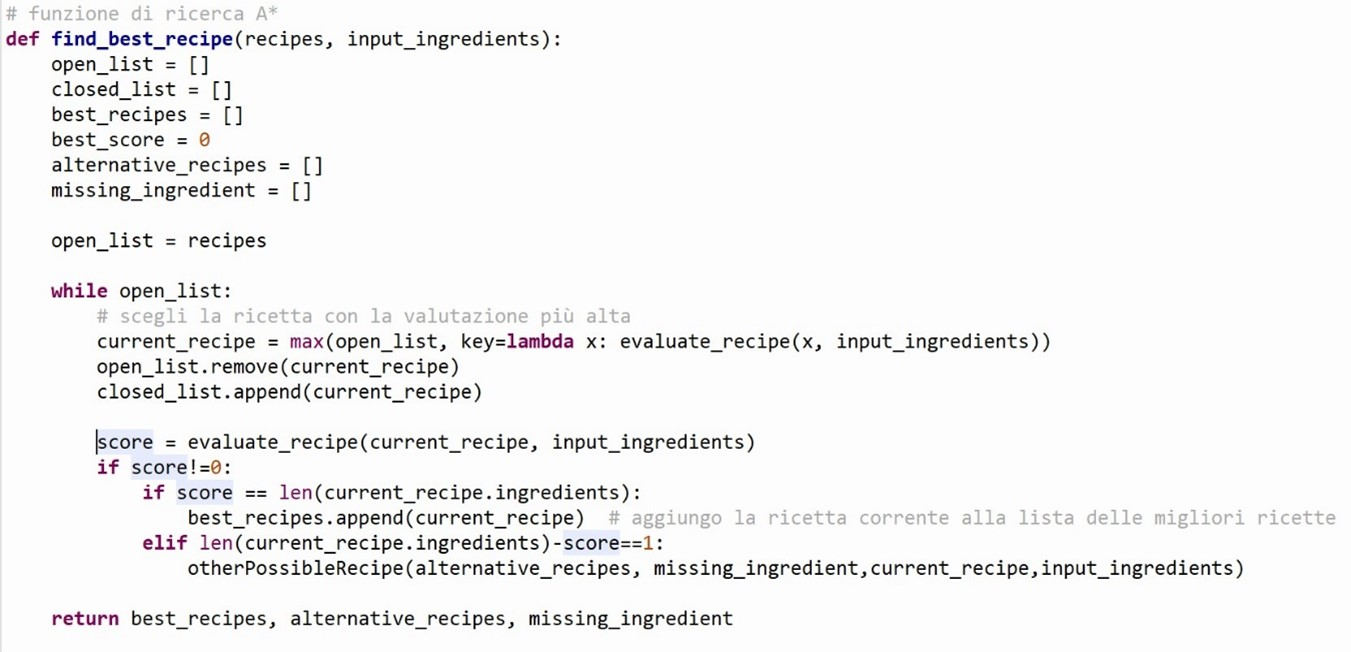
\includegraphics[width=0.9\textwidth]{img/img11.jpg}}
\end{figure}

Il programma funzionava abbastanza bene riusciva a dare in output le ricette che ottimizzavano gli ingredienti forniti in input ed anche le ricette a cui mancava un solo ingredienti di quelli a disposizione. 

\begin{figure}[H]
        \centering
        {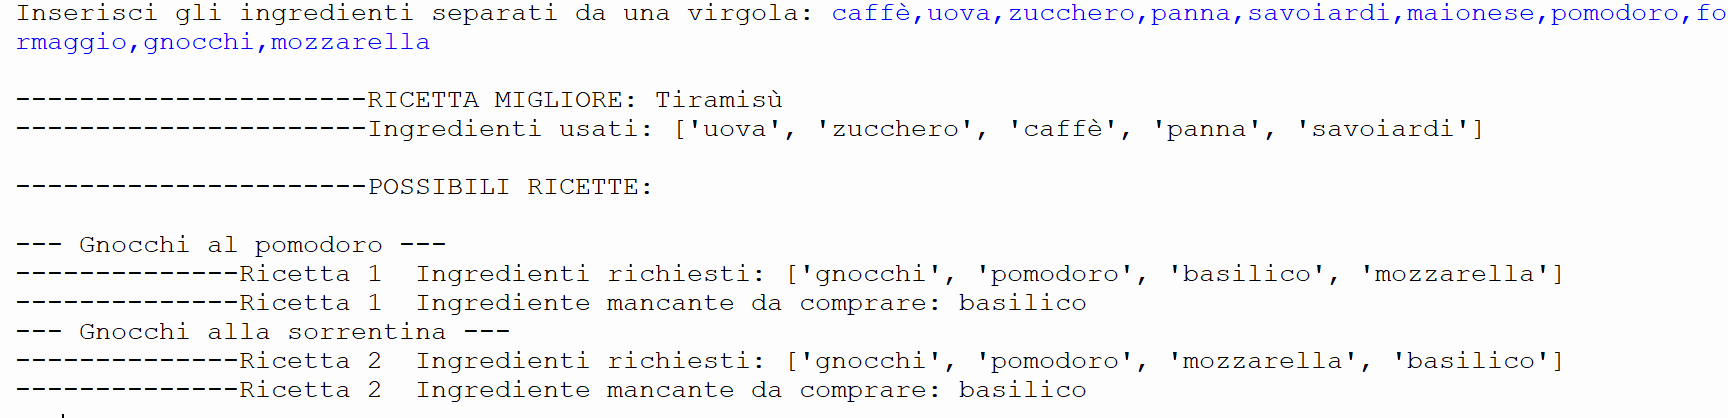
\includegraphics[width=0.9\textwidth]{img/img33.jpg}}
\end{figure}

Il problema era che era troppo troppo lento, già con un dataset piccolo, inoltre, anlaizando meglio il codice ci siamo accorti che probabilmente era una semplice ricerca e non un algoritmo A Star, in quanto non utilizza h(n).

\chapter{Terza Soluzione TF-IDF + similiarità del coseno}

Facendo un paio di ricerche sul web abbiamo compreso che il nostro era un problema facente parte del NLP, una branca dell’AI.
Nello specifico un Probelma di Text Classification, ovvero identificare gli argomenti di un testo nel nostro caso gli ingredienti delle ricette e la loro correlazione.

Per poter risolvere i problemi di Text Classification si può utilizzare il word embedding.

\section{Word Embedding} 

La semplice definizione di word embedding è la conversione di testo in numeri. Per far sì che il computer capisca il linguaggio, convertiamo il testo in forma vettoriale in modo che i computer possano sviluppare connessioni tra i vettori e le parole e capire ciò che diciamo. Con il word embedding, risolviamo i problemi relativi al Natural Language Processing.

Le rappresentazioni vettoriali dei tokens, chiamate Word Embeddings, sono apprese da modelli NLP, definiti come modelli spaziali vettoriali

Le singole parole sono analizzate e rappresentate atomicamente come unità singole in 
\textbf{Bag-of-Words} (BOW): questo ‘bagaglio’ di parole, o ‘set’, sono una rappresentazione sparsa delle parole e della loro presenza, indipendentemente dall'ordine sintattico in cui appaiono in una data frase.

L'idea è molto semplice: ogni documento del nostro corpus viene rappresentato contando quante volte ogni parola appare in esso.
Ad esempio se prendiamo due ricette e quindi due liste di ingredienti(documenti) 

R1 Tiramisù : "mascarpone,uova,savoiardi,zucchero,caffè,cacao”

R2 Spaghetti alla Carbonara :"spaghetti,guanciale,uova,pecorino,pepe” 

\begin{center}
\resizebox{\columnwidth}{!}{\begin{tabular}{|c|c|c|c|c|c|c|c|c|c|c|} 
 \hline
 & mascarpone & uova & savoiardi & zucchero & caffè & cacao & spaghetti & guanciale & pecorino & pepe \\ [0.5ex] 
 \hline
R1  & 1 & 1 & 1 & 1 & 1 & 1 & 0 & 0 & 0 & 0\\
 \hline
R2  & 0 & 1 & 0 & 0 & 0 & 0 & 1 & 1 & 1 & 1\\
 \hline
\end{tabular}}
\end{center}

Questa viene chiamata matrice documento-caratteristica (document-feature matrix): ogni riga rappresenta un diverso documento (ricetta) e ogni colonna definisce la caratteristica usata per rappresentare il documento

Nel nostro dataset abbiamo circa 560 ingredienti diversi, quindi il modello bag of word crea un'enorme matrice sparsa che memorizza i conteggi di tutte le parole nel nostro corpus (tutti i documenti, ovvero tutti gli ingredienti per ogni ricetta). Per farlo praticamente si puo utilizzare CountVectorizer della libreria scikit-learn (questa libreria la useremo spesso nel nostro discorso)

Bag of Words crea solo un insieme di vettori contenente il conteggio delle occorrenze di parole nelle frasi/corpus, ma non contiene informazioni su parole importanti.

\section{TF-IDF}

Continuando nelle ricerche abbiamo trovato un altro metodo chiamato TF-IDF (term frequencies- inverse document frequency). Che ha lo scopo di riflettere quanto sia rilevante un termine in un dato documento.

TF-IDF è una tecnica nell'elaborazione del linguaggio naturale per convertire le parole in vettori e con alcune informazioni semantiche e dà peso a parole non comuni, utilizzate in varie applicazioni di NLP. 

Ad esempio sale , olio sono presenti in più del 60\% delle ricette quindi non sono molto rilevanti al fine di determinare la similitudine tra due ricette. TF-IDF assegnerà un valore più basso al sale.
Per una spiegazione più precisa del funzionamento di TF-IDF vedere il seguente link \href{https://medium.datadriveninvestor.com/tf-idf-in-natural-language-processing-8db8ef4a7736}{medium.datadriveninvestor}.

Per usare TF-IDF in python si utilizza TfidfVectorizer della libreria sk-learn 

La libreria scikit-learn TfidfVectorizer esegue un processo di tokenizzazione dei testi per separare le parole individuali (o le frasi) nei documenti di testo e quindi costruisce una matrice di term frequency-inverse document frequency (TF-IDF) come descritto sopra

La matrice TF-IDF è utilizzata per rappresentare i documenti (ricette) come un insieme di features (ingredienti) in un formato che può essere utilizzato come input per i modelli di machine learning.

\begin{figure}[H]
        \centering
        {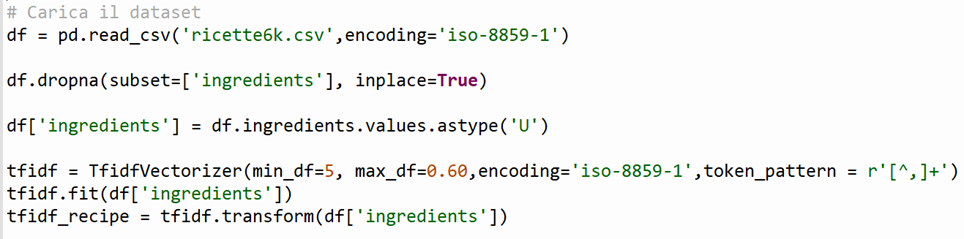
\includegraphics[width=0.9\textwidth]{img/img12.jpg}}
\end{figure}

max\_df non considera le parole che sono presenti più del 60\% 

token\_pattern = r'[\^,]+: Questa regex matcha una qualsiasi serie di caratteri che non sia una virgola

Il modello TF-IDF viene addestrato sull'intero dataset di ingredienti utilizzando il metodo fit().

Il modello viene quindi utilizzato per trasformare questi ingredienti in una rappresentazione numerica utilizzando il metodo transform(). Questa rappresentazione viene chiamata "codifica TF-IDF".

Per Misurare la somiglianza tra le liste degli ingredienti e gli ingredienti dati in input abbiamo utilizzato la Similarità del coseno, funzione di Sklearn con le stesse somiglianze e per i dati testuali viene utilizzata per trovare la somiglianza di testi nel documento. 
Viene usata la funzione ottieni consigli per classificare i punteggi e generare un dataframe, tramite la libreria pandas, contente il titolo, gli ingredienti e il punteggio delle ricette consigliate.

La similarità del coseno è una misura della somiglianza tra due punti dati in un piano. La somiglianza del coseno viene utilizzata per determinare la distanza tra i vicini, ad esempio nei sistemi di raccomandazione viene utilizzata per consigliare film .

I risultati ottenuti sono accettabili ma molte volte consiglia delle ricette per niente simili.

Per migliorarlo avevamo bisogno di tenere traccia degli ingredienti comunemente usati insieme. 

\section{Word2vec}

IL nostro problema era: Come facciamo a far comprendere all’agente intelligente che alcuni ingredienti stanno bene insieme dato che sono presenti delle ricette nel dataset in cui compaio gruppi di ingredienti insieme?
Per fare questo abbiamo addrestrato un modello chiamtao Word2vec in quanto è  altamente efficiente nel raggruppare insieme parole simili.

Per esempio i pomodori sono simili ad altri ingredienti usati spesso insieme. 

\begin{figure}[H]
        \centering
        {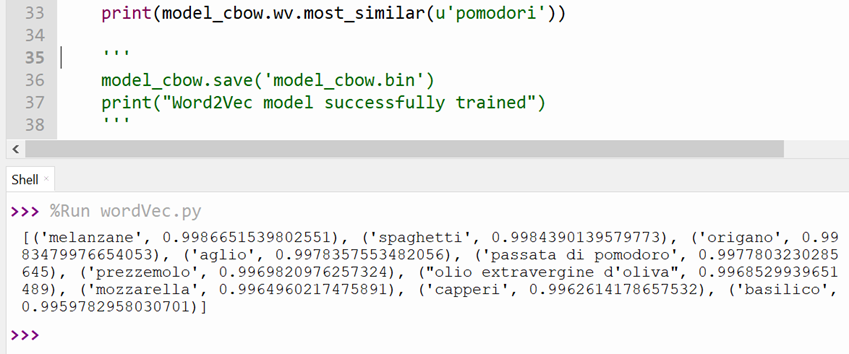
\includegraphics[width=0.9\textwidth]{img/img13.jpg}}
\end{figure}

Word2vec è una semplice rete neurale artificiale a due strati progettata per elaborare il linguaggio naturale, l'algoritmo richiede in ingresso un corpus e restituisce un insieme di vettori che rappresentano la distribuzione semantica delle parole nel testo.

Per addestrare il modello, lo strato di input includerà il numero di neuroni pari alle parole del vocabolario. La dimensione dello strato di uscita e dello strato di ingresso rimane la stessa. Tuttavia, la dimensione dello strato nascosto è impostata in base ai vettori delle dimensioni delle parole risultanti. È possibile eseguire l’incorporazione di parole con Word2Vec attraverso due metodi. In entrambi i metodi sono necessarie reti neurali artificiali. Questi metodi sono: 

\begin{itemize}
\item \textbf{CBOW : } è denominato metodo “Continuous Bag of Words” (CBOW), per predire una parola target basata su una sequenza contigua di n-grammi.
\item \textbf{Skim Gram : } usa un vettore di parole per predire un contesto target
\end{itemize}

Nel nostro caso abbiamo usato CBOW

Per realizzarlo in python abbiamo usato la libreria gensim e seguito alcune guide online come questa: \href{http://nadbordrozd.github.io/blog/2016/05/20/text-classification-with-word2vec/}{guida}.

Dovevamo rappresentare ogni documento corpus (lista di ingredienti per ricetta) come un singolo incorporamento in modo tale da calcolare le somiglianze.

Di seguito il codice per allenare il modello Word2Vec

\begin{figure}[H]
        \centering
        {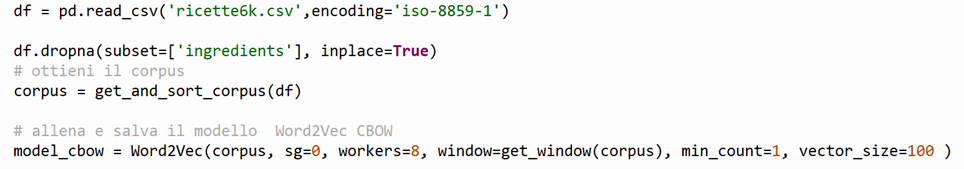
\includegraphics[width=0.9\textwidth]{img/img14.jpg}}
\end{figure}

\begin{itemize}
	\item Vector\_size= n, permette di decidere la dimensione dei vettori che l'algoritmo andrà a creare.
	\item window= n, permette di decidere la massima distanza tra la parola corrente e quella predetta all'interno di una frase. Nel nostro caso è dato dalla media di ingredienti in una ricetta (9)
	\item min\_count=n, utile per capire se una determinata ricetta piace agli utenti o meno (non verrà usata nella soluzione finale)
	\item workers= n, permette di decidere quanti thread del processore usare per addestrare il modello.
	\item sg= o, questo crea un modello CBOW
 \end{itemize}

Usiamo TD-IDF per aggregare gli accorpamenti.

Calcoliamo la media ponderata di tutti gli incorporamenti di parole di ogni documento(lista ingredienti) e ridimensioniamo ogni vettore usando la sua frequenza inversa del documento (IDF).

IDF appesantirà i termini molto comuni in un corpus (nel nostro caso parole come olio extravergine d'oliva o sale e soppeserà i termini rari.

In questo modo si ha una capacità di separare le ricette migliore.

Word2Vec cerca di prevedere le parole in base all'ambiente circostante, quindi era fondamentale ordinare gli ingredienti in ordine alfabetico

\begin{figure}[H]
        \centering
        {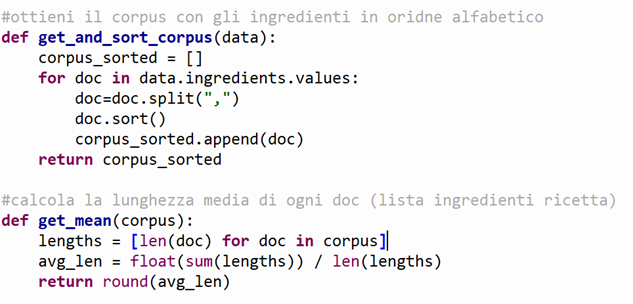
\includegraphics[width=0.9\textwidth]{img/img15.jpg}}
\end{figure}

Abbiamo poi utilizzato sia la similarità del  sia knn per trovare le ricette simili.

\section{Similarità del coseno}

La similarità del coseno : 

\begin{figure}[H]
        \centering
        {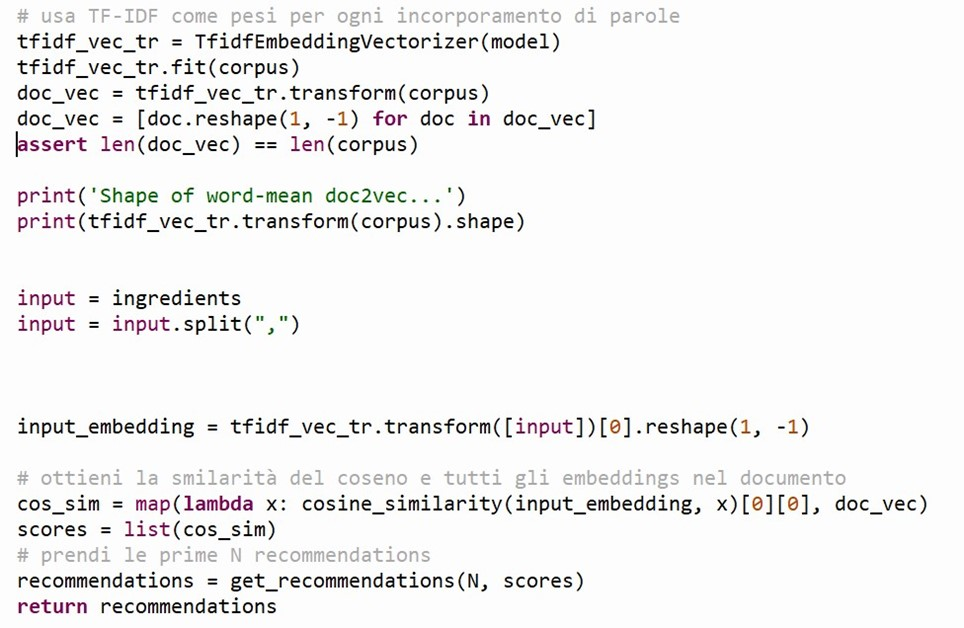
\includegraphics[width=0.9\textwidth]{img/img16.jpg}}
\end{figure}

\section{KNN}

Abbiamo testato il funziomento anche con  KNN.

Il k-nearest neighbors (traducibile come primi k-vicini), abbreviato in K-NN, è un algoritmo utilizzato nel riconoscimento di pattern per la classificazione di oggetti basandosi sulle caratteristiche degli oggetti vicini a quello considerato.

In questo caso abbiamo usato KNN per trovare le ricette più vicine rispetto a agli ingredienti che l'utente ha fornito. Per fare questo, prima abbiamo convertito i nomi degli ingredienti in vettori utilizzando un modello di embedding. Questi vettori hanno una rappresentazione in uno spazio a più dimensioni che rappresenta la somiglianza semantica degli ingredienti.

Successivamente, abbiamo calcolato la distanza tra il vettore di embedding della ricetta dell'utente e il vettore di embedding di ogni ricetta nella nostra base di dati utilizzando la distanza Euclidea. Infine, abbiamo selezionato le K ricette più vicine (dove K è un parametro che possiamo impostare) e abbiamo restituito i nomi di queste ricette come raccomandazioni, usando la funzione get\_recommendations.

In sintesi, KNN è stato utilizzato per trovare le ricette più simili a quella fornita dall'utente utilizzando la distanza Euclidea tra i vettori di embedding degli ingredienti.

Codice: 

\begin{figure}[H]
        \centering
        {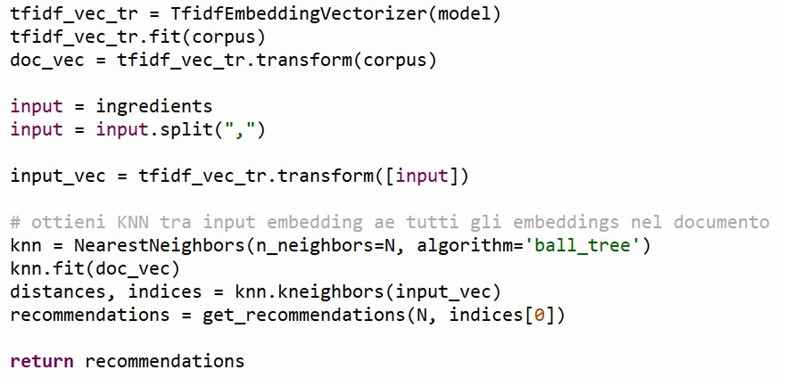
\includegraphics[width=0.9\textwidth]{img/img17.jpg}}
\end{figure}

La riga knn = NearestNeighbors(n\_neighbors=N, algorithm='ball\_tree') crea un oggetto di tipo NearestNeighbors da scikit-learn.

 La classe NearestNeighbors ha due parametri importanti: 
\begin{itemize}
\item n\_neighbors: questo parametro specifica il numero di vicini più vicini che vogliamo trovare per ogni punto del dataset. In questo caso, n\_neighbors=N significa che stiamo cercando i N vicini più vicini.
\item algorithm: questo parametro specifica l'algoritmo di ricerca delle vicinanze che si desidera utilizzare. Nel caso specifico, l'algoritmo specificato è 'ball\_tree'.
\end{itemize}
Il modello viene addestrato sulla matrice dei vettori dei documenti con il metodo fit. Infine, il metodo kneighbors viene utilizzato per ottenere le K (in questo caso, N) vicinanze più vicine tra il vettore di input e tutti i vettori dei documenti.

Metriche valutazione KNN:

\begin{figure}[H]
        \centering
        {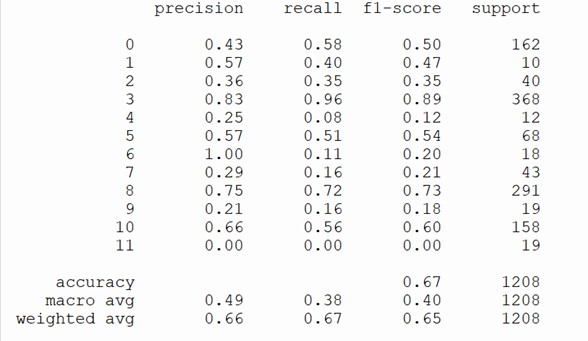
\includegraphics[width=0.9\textwidth]{img/img21.jpg}}
\end{figure}

KNN: input: "farina,uova,grana padano,pangrattato"

\begin{figure}[H]
        \centering
        {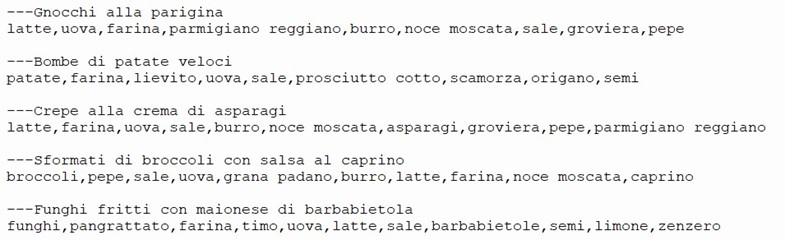
\includegraphics[width=0.9\textwidth]{img/img18.jpg}}
\end{figure}

Per cos\_sim non è possibile valutare tramite precision, recall, ecc . Ci siamo basati su Score

COS\_SIM: input "farina,uova,grana padano,pangrattato"

\begin{figure}[H]
        \centering
        {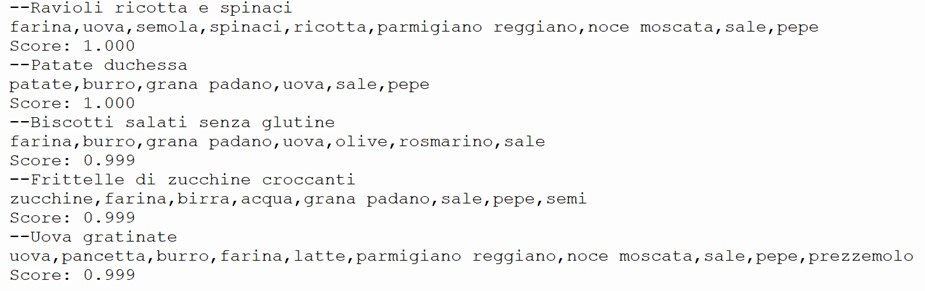
\includegraphics[width=0.9\textwidth]{img/img19.jpg}}
\end{figure}

\chapter{Quarza Soluzione : Clustering}

Abbiamo poi ripreso la soluzione che usava sono TD-IDF e cosine\_similarity e abbiamo usato la cosine\_similarity come input per un algoritmo di clustering. Ed il risultato è stato ottimo.

Per il clustering abbiamo scelto l’algoritmo K-Means uno dei più diffusi.
Attuando due strategie: 

Nella prima stategia abbiamo calcolato la cosine\_similarity di tra tutte le ricette del dataset a priori e l'abbiamo passata in input al clustering.

Nel seconda strategia abbiamo creato il clustering una volta calcolato la cosine\_similarity tra la ricetta scelta e tutte le altre ricette del dataset.

Per la scelta del K abbiamo usato in entrambe le strategie il metodo dell’elbow point per la scelta del k, e Il Silhouette Coefficient per la bontà dei claster.

L'elbow point è una metrica nell'analisi del cluster per determinare il numero ottimale di cluster da utilizzare in un modello di clustering. Il punto gomito rappresenta il numero di cluster in cui l'incremento della somma delle distanze quadratiche medie (SSE, Sum of Squared Errors) tra i punti del cluster e il centroide del cluster stesso, inizia a rallentare. 

Questo punto viene identificato come il punto in cui l'aggiunta di ulteriori cluster non apporta un significativo miglioramento del modello. In altre parole, l'elbow point rappresenta la trade-off tra il numero di cluster e la qualità del modello di clustering

Silhouette Coefficient è una metrica che valuta la qualità di un clustering rispetto a come le osservazioni sono state assegnate ai vari cluster. Un valore più alto indica un clustering di qualità superiore, con valori compresi tra -1 e 1.

\section{Prima Strategia}   

Elbow Point

\begin{figure}[H]
        \centering
        {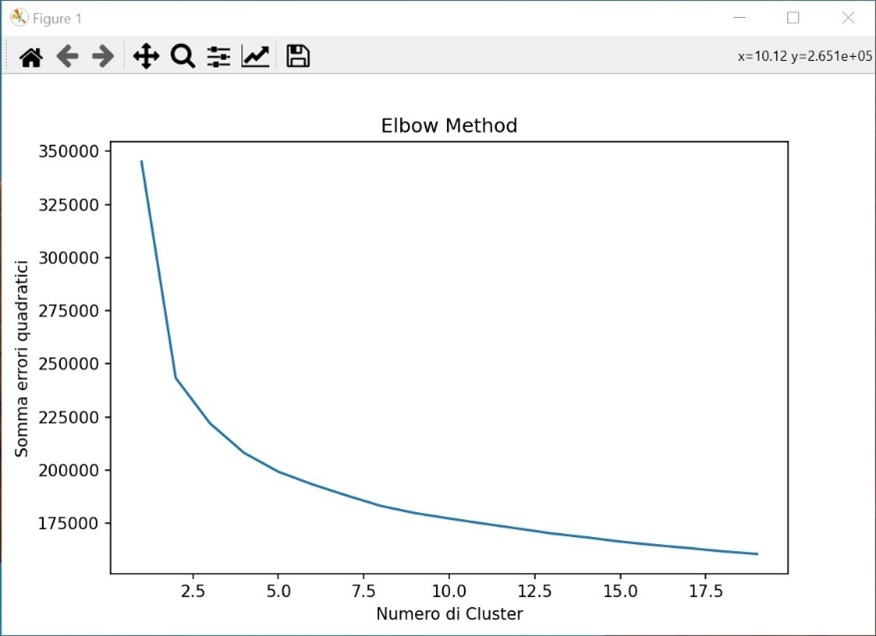
\includegraphics[width=0.7\textwidth]{img/img22.jpg}}
\end{figure}

Cluster

\begin{figure}[H]
        \centering
        {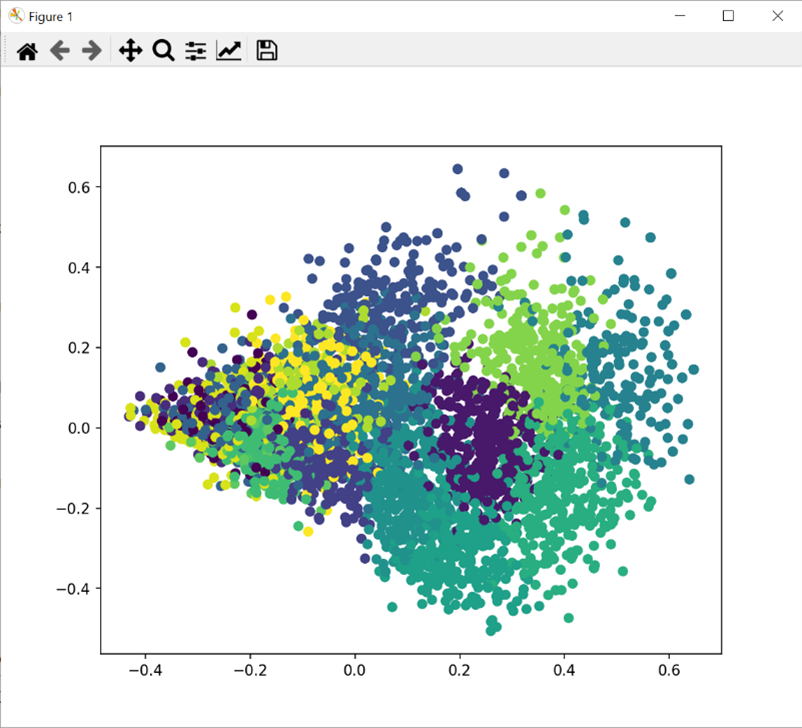
\includegraphics[width=0.7\textwidth]{img/img23.jpg}}
\end{figure}

Output fissato a 10
\begin{figure}[H]
        \centering
        {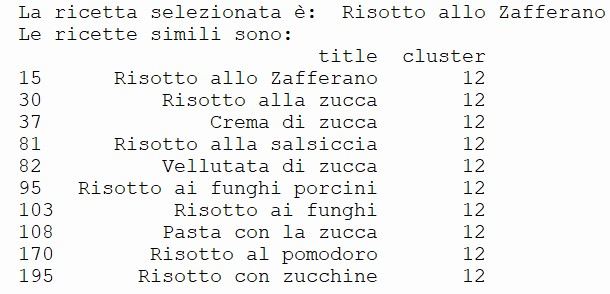
\includegraphics[width=0.7\textwidth]{img/img24.jpg}}
\end{figure}

Silhouette Coefficient

\begin{figure}[H]
        \centering
        {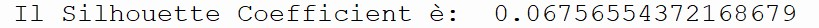
\includegraphics[width=0.7\textwidth]{img/img28.jpg}}
\end{figure}

\section{Seconda Strategia}   

Elbow Point

\begin{figure}[H]
        \centering
        {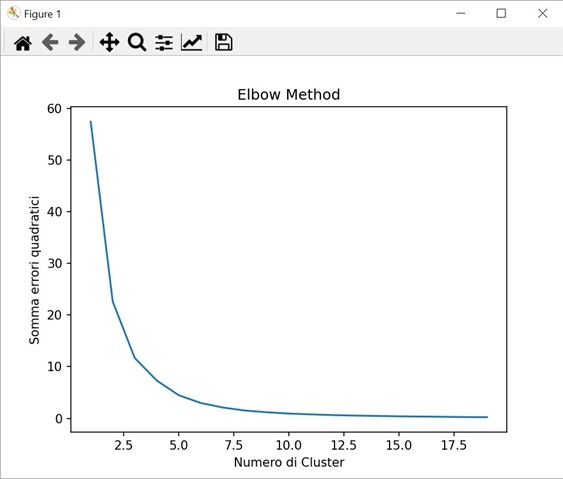
\includegraphics[width=0.7\textwidth]{img/img25.jpg}}
\end{figure}

Abbiamo visto che già con 5 il risultato era ottimo.

Cluster

\begin{figure}[H]
        \centering
        {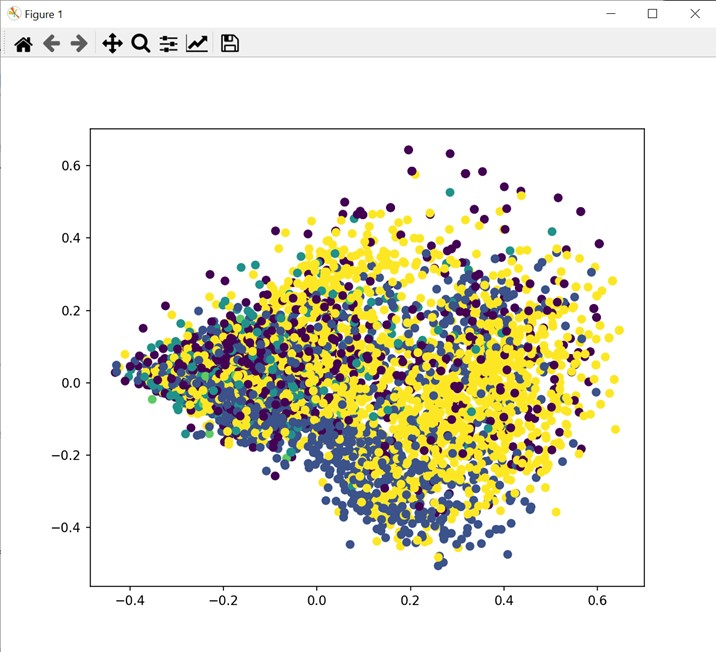
\includegraphics[width=0.7\textwidth]{img/img26.jpg}}
\end{figure}

Output fissato a 10

\begin{figure}[H]
        \centering
        {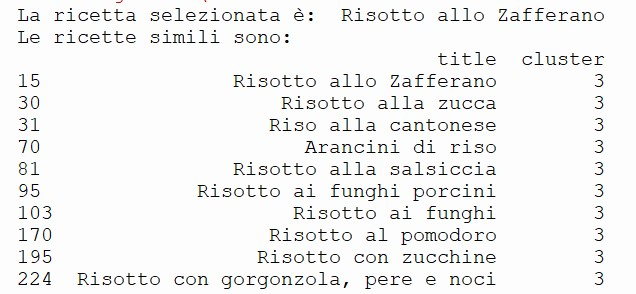
\includegraphics[width=0.7\textwidth]{img/img27.jpg}}
\end{figure}

Silhouette Coefficient

\begin{figure}[H]
        \centering
        {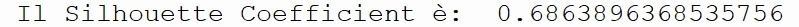
\includegraphics[width=0.7\textwidth]{img/img29.jpg}}
\end{figure}

Con la prima posiamo effettuare il clustering una sola volta, salvare nel dataset per ogni ricetta il suo cluster di appartenenza, e quindi azzerare quasi del tutto il tempo di attesa del risultato.
Con la seconda però abbiamo raccomandazioni più precise , vedi il silhouette Coefficient

\chapter{App}
Per creare l’interfaccia grafica dell’applicazione abbiamo usato la libreria customtkinter di python che permette di creare una gui semplice e minimale. Inoltre è possibile non solo inserire una serie di ingredienti che abbiamo , ma anche selezionare a video delle ricette che ci piacciono per farci consigliare altre ricette simili. 
\section{GUI}
 Nella pagina iniziale vengono mostrate una serie di ricette che l'utente può selezionare, e per ognuna delle quali il programma restituisce 4 ricette consigliate.
 L'utente può anche scrivere gli ingredienti che ha disposizione nel campo di testo o dirli a voce  selezionando il bottone "mic".

Inoltre può selezionare con quale strategia effettuare la ricerca (Word2Vec, Clustering 1, Clustering 2)
 
 Una volta che ha selezionato una ricetta e/o inserito degli ingredienti può procedere con il premere "Avvia Ricerca".
 Se non vede nessuna ricetta che gli piace può generarne di nuove con il bottone "Nuove ricette", oppure dopo che ha ottenuto dei cosigli su una ricetta può tornare alla stessa lista di ricette con il bottone "Lista ricette" per selezionarne una che aveva dimenticato.
 

\begin{figure}[H]
        \centering
        {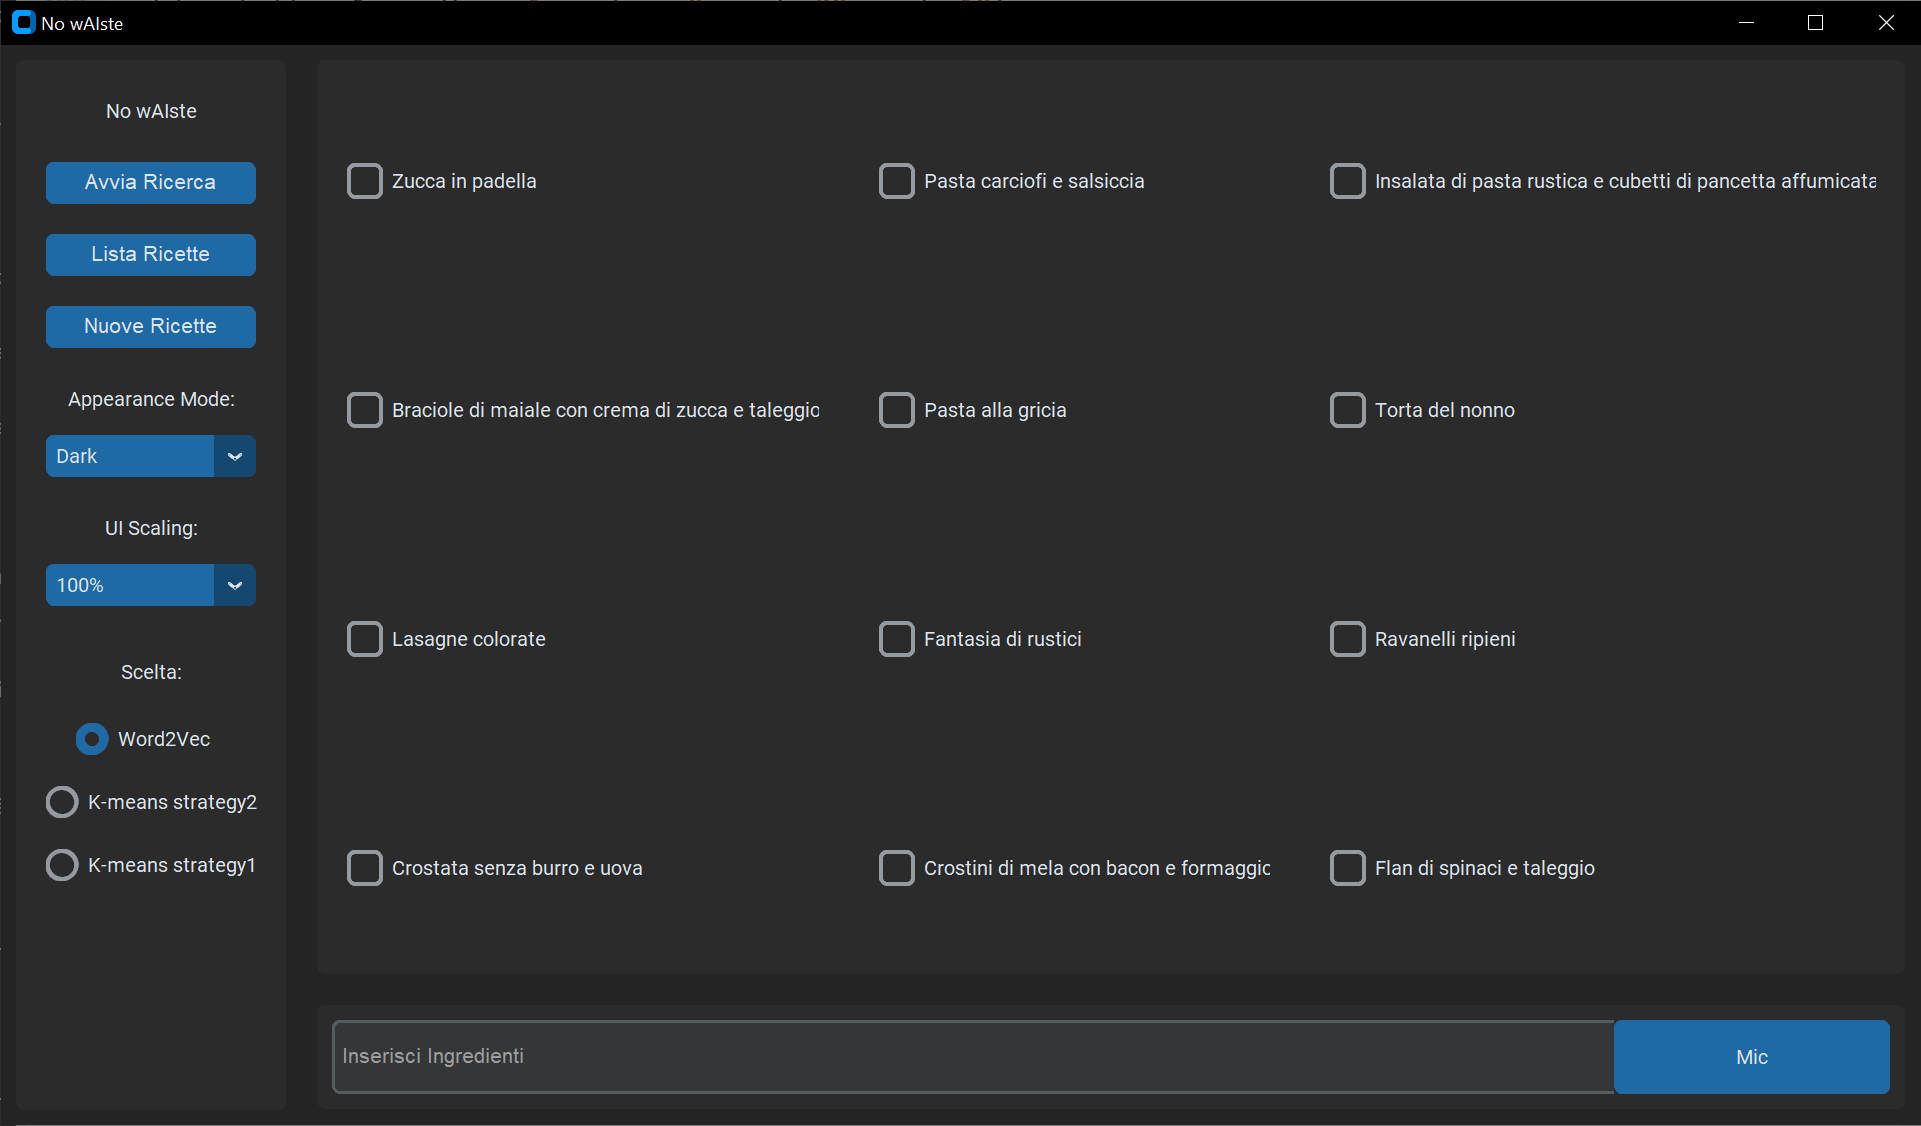
\includegraphics[width=0.9\textwidth]{img/img32.jpg}}
\end{figure}

\begin{figure}[H]
        \centering
        {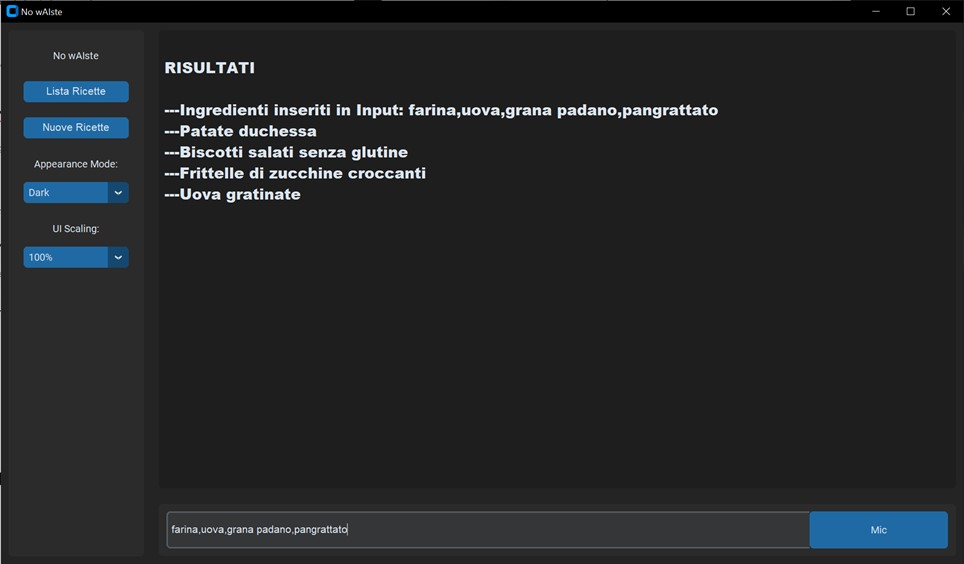
\includegraphics[width=0.9\textwidth]{img/img31.jpg}}
\end{figure}

\section{Input Vocale}   
\begin{figure}[H]
        \centering
        {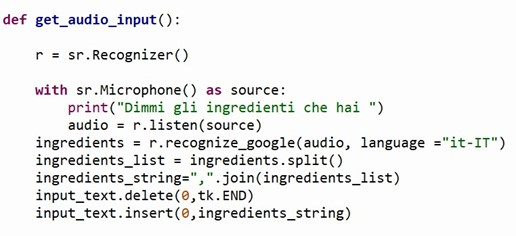
\includegraphics[width=0.9\textwidth]{img/img20.jpg}}
\end{figure}

Questo codice è una funzione chiamata "get\_audio\_input" che utilizza la libreria "SpeechRecognition" (sr) per riconoscere la voce dell'utente e tradurla in testo. La funzione utilizza un microfono come fonte di input audio. Quando l'utente inizia a parlare, il codice registra l'audio e lo passa al metodo "recognize\_google" dell'oggetto "Recognizer" per ottenere la traduzione in testo. Il risultato viene salvato come stringa in "ingredients". Successivamente, la stringa viene divisa in una lista di parole utilizzando il metodo "split" e la lista viene successivamente trasformata in una stringa separata da virgole utilizzando il metodo "join". Infine, il testo viene inserito nella casella di testo visualizzata sull'interfaccia utente.

\chapter{Riferimenti}

\begin{itemize}
\item Word2Vec  : \href{http://nadbordrozd.github.io/blog/2016/05/20/text-classification-with-word2vec/}{link}, \href{https://github.com/TomLin/Playground/blob/master/04-Model-Comparison-Word2vec-Doc2vec-TfIdfWeighted.ipynb}{link} , \href{https://towardsdatascience.com/an-introduction-to-word2vec-in-nlp-854e1c288894}{link}.
\item NLP: \href{https://towardsdatascience.com/nlp-performance-of-different-word-embeddings-on-text-classification-de648c6262b}{link}.
\item Web Scraping : \href{https://realpython.com/beautiful-soup-web-scraper-python/}{link}.
\item Libreria python : \href{ https://github.com/hhursev/recipe-scrapers}{link}.
\end{itemize}

\end{document}
